\documentclass[x11names,a4paper,12pt]{article}
\usepackage[brazil]{babel}
\usepackage[utf8]{inputenc}
\usepackage{graphicx}
\usepackage{pgfplots}
\usepackage{tikz}
\usepackage{float}
\usepackage{xcolor}
\usepackage{amsmath}
\usepackage{amssymb}
\usepackage{hyperref}
\usepackage{minted}

\hypersetup{
    colorlinks=true,
    linkcolor=black,
    filecolor=black,
    urlcolor=blue,
}

\pgfplotsset{compat=1.16}

\usetikzlibrary{shapes.geometric,arrows}

\tikzstyle{startstop} = [rectangle,
                         rounded corners,
                         minimum width=3cm,
                         minimum height=1cm,
                         text centered,
                         draw=black,
                         fill=red!30]

\tikzstyle{process} = [rectangle,
                       minimum width=3cm,
                       minimum height=1cm,
                       text centered,
                       text width=3cm,
                       draw=black,
                       fill=orange!30]

\tikzstyle{decision} = [diamond,
                        minimum width=3cm,
                        minimum height=1cm,
                        text centered,
                        draw=black,
                        fill=green!30]

\tikzstyle{arrow} = [thick,
                      ->,
                      >=stealth]

\title{Exercício de Fixação de Conceitos (EFC) 1 – Sistemas LIT e Resposta em Frequências}
\author{George Nicolas Kontogiorgos}
\date{\today}

\begin{document}

\maketitle

\tableofcontents

\section{Parte teórica}

\subsection{Determinação do comprimento P} \label{ssec:p_length}

Podemos determinar o comprimento $P$ da sequência $y[n]$ gerada na saída do sistema em função de $K$ e $D$, comprimentos da entrada $x[n]$ e da resposta ao impulso $h[n]$ respectivamente, com o método de cálculo analítico da convolução. Tal procedimento faz referência ao exemplo dado em aula pelo professor e ao exemplo 11 do capítulo 2 do  livro texto. A operação de convolução é dada por

\begin{equation}
  y[n]=x[n]*h[n]=\sum_{k=-\infty}^{\infty}{x[k]h[n-k]}
  \label{eqn:discrete_convolution}
\end{equation}

Iniciamos o processo operando sobre a resposta ao impulso. O objetivo é obter $h[n-k]$ neste primeiro momento. A função de resposta ao impulso pode ser esboçada (como sugere o enunciado) por:

\begin{figure}[H]
  \centering
  \begin{tikzpicture}[scale=1]
    \begin{axis}[axis lines=middle,x=1cm, xtick={1,...,3,5},
      xticklabels={{}, {}, 3, $D-1$},
      extra x ticks={1, 2},
      extra x tick labels={$1$, $2$},
      extra x tick style={
        xticklabel style={yshift=0.5ex, anchor=south}},
      xmin=0,xmax=6, ytick={\empty}, yticklabels={},
      ymin=-4, ymax=6, axis on top]
      \addplot+[ycomb, blue, thick, mark=*, mark options={blue}] plot coordinates
      {(0,0) (1,-3) (2,-1) (3,1) (5,5)};
    \end{axis}
    \node at (4cm,2.5) {$\cdots$};
    \node at (-0.5,2.6) {\textcolor{blue}{$h[0]$}};
    \node at (1cm,0.2) {\textcolor{blue}{$h[1]$}};
    \node at (2,1.3) {\textcolor{blue}{$h[2]$}};
    \node at (3,3.2) {\textcolor{blue}{$h[3]$}};
    \node at (5,5.5) {\textcolor{blue}{$h[D-1]$}};
    \node at (6.1,2.5) {$k$};
    \node at (0,6) {$h[k]$};
  \end{tikzpicture}
  \caption{Resposta ao impulso.}
  \label{fig:impulse_respose}
\end{figure}

Espelhamos o sinal

\begin{figure}[H]
  \centering
  \begin{tikzpicture}[scale=1]
    \begin{axis}[axis lines=middle, xtick={-5,-3,...,-1,0},
      xticklabels={$-(D-1)$, -3, {}, {}, 0},
      extra x ticks={-2, -1},
      extra x tick labels={$-2$, $-1$},
      extra x tick style={
        xticklabel style={yshift=0.5ex, anchor=south}},
      xmin=-6,xmax=1, ytick={\empty}, yticklabels={},
      ymin=-4,  ymax=6, axis on top]
      \addplot+[ycomb, blue, thick, mark=*, mark options={blue}] plot coordinates
      {(0,0) (-1,-3) (-2,-1) (-3,1) (-5,5)};
    \end{axis}
    \node at (2,2.5) {$\cdots$};
    \node at (7,2.5) {$k$};
    \node at (6,6) {$h[-k]$};
  \end{tikzpicture}
  \caption{Resposta ao impulso espelhada.}
  \label{fig:h_flipped}
\end{figure}

e efetuamos um deslocamento de $n$ amostras e forma-se o sinal $h[n-k]$

\begin{figure}[H]
  \centering
  \begin{tikzpicture}[scale=1]
    \begin{axis}[axis lines=middle, x=1cm, xtick={0,2,4,5,6,7},
      xticklabels={0,\footnotesize{$n-(D-1)$}, \footnotesize{$n-3$}, {}, {}, \footnotesize{$n$}},
      extra x ticks={5, 6},
      extra x tick labels={\footnotesize{$n-2$}, \footnotesize{$n-1$}},
      extra x tick style={
        xticklabel style={yshift=0.5ex, anchor=south}},
      xmin=0,xmax=8, ytick={\empty}, yticklabels={},
      ymin=-4,  ymax=6, axis on top]
      \addplot+[ycomb, blue, thick, mark=*, mark options={blue}] plot coordinates
      {(2,5) (4,1) (5,-1) (6,-3) (7,0)};
    \end{axis}
    \node at (1cm,2.5) {$\cdots$};
    \node at (3cm,2.5) {$\cdots$};
    \node at (8.1cm,2.5) {$k$};
    \node at (0,6) {$h[n-k]$};
  \end{tikzpicture}
  \caption{Resposta ao impulso espelhada e deslocada de $n$ amostras.}
  \label{fig:h_flipped_shifted}
\end{figure}

Neste segundo momento iremos avaliar os extremos da convolução discreta. Para isso, analisaremos, primeiramente $n=0$, posição que a resposta ao impulso “toca” o sinal de entrada

\begin{figure}[H]
  \centering
  \begin{tikzpicture}[scale=1]
    \begin{axis}[axis lines=middle, x=1cm, y=0.5cm, xtick={-5,-3,...,-1,0,1,2,4},
      xticklabels={$-(D-1)$, -3, {}, {}, 1, {}, $K-1$},
      extra x ticks={-2, -1, 2},
      extra x tick labels={$-2$, $-1$, $2$},
      extra x tick style={
        xticklabel style={yshift=0.5ex, anchor=south}},
      xmin=-6,xmax=5, ytick={\empty}, yticklabels={},
      ymin=-4,  ymax=6, axis on top]
      \addplot+[ycomb, blue, thick, mark=*, mark options={blue}] plot coordinates
      {(-5,5) (-3,1) (-2,-1) (-1,-3) (0,0)};
      \addplot+[ycomb, red, thick, mark=x, mark options={red}] plot coordinates
      {(0,2) (1,3) (2,-1.4) (4,4)};
    \end{axis}
    \node at (2,2.3) {$\cdots$};
    \node at (9,2.3) {$\cdots$};
    \node at (11,2.3) {$k$};
    \node at (6,5.2) {\textcolor{blue}{$h[n-k]$}, \textcolor{red}{x[k]}};
  \end{tikzpicture}
  \caption{Primeira posição do deslocamento no processo de convolução.}
  \label{fig:begin_convolution}
\end{figure}

Desta imagem podemos notar que $n<0$ implica $y[n]=0$ uma vez que um nessas regiões os produtos das amostras da resposta ao impulso com a entrada seriam nulas. Isso se dá porque $x[n]=0$ para $n<0$, por definição do sinal.
O outro extremo pode ser analisado por partes. Imagine primeiramente que o deslocamento será de $n=K-1$. Nessa condição, a amostra $h[0]$ coincidirá com a amostra $x[K-1]$. Com essa intuição, podemos imaginar então a segunda parte do raciocínio, quando a amostra $h[D-1]$ coincida com $x[K-1]$. Essa será o outro extremo do cálculo da convolução. Para que essa situação ocorra, teremos que fazer o deslocamento ser $n=K+D-2$. Segue o gráfico dessa última condição:

\begin{figure}[H]
  \centering
  \begin{tikzpicture}[scale=1]
    \begin{axis}[
      axis lines=center,
      x=1.5cm,
      y=0.5cm,
      xtick={0,1,2,3,4,5,6,7},
      xticklabels={0, 1, {}, \tiny{$K-1$}, \tiny{$K+D-5$}, {}, {}, \tiny{$K+D-2$}},
      extra x ticks={2, 5, 6},
      extra x tick labels={$2$, \tiny{$K+D-4$}, \tiny{$K+D-3$}},
      extra x tick style={xticklabel style={yshift=0.5ex, anchor=south}},
      xmin=0,
      xmax=8,
      ytick={\empty},
      yticklabels={},
      ymin=-4,
      ymax=6,
      axis on top]
      \addplot+[ycomb, blue, thick, mark=*, mark options={blue}] plot coordinates
      {(3,5) (4,1) (5,-1) (6,-3) (7,0)};
      \addplot+[ycomb, red, thick, mark=x, mark options={red}] plot coordinates
      {(0,2) (1,3) (2,-1.4) (3,4)};
    \end{axis}
    \node at (3.75cm,2.3) {$\cdots$};
    \node at (5.25cm,2.3) {$\cdots$};
    \node at (12cm,2.3) {$k$};
    \node at (0,5.2) {\textcolor{blue}{$h[n-k]$}, \textcolor{red}{x[k]}};
  \end{tikzpicture}
  \caption{Última posição do deslocamento no processo de convolução.}
  \label{fig:end_convolution}
\end{figure}

Note que com um incremento unitário no deslocamento todos os produtos se anulam, como no caso de $n<0$. Dado isso, temos também $y[n]=0$ para $n>K+D-2$, e, podemos escrever, de uma forma mais ampla:

\begin{equation}
  y[n] =
  \begin{cases}
    x[n]*h[n], & 0 \leq n \leq K+D-2\\
    0        , & caso\ contr\acute{a}rio
  \end{cases}
\end{equation}

Fica evidente dessa análise que o comprimento temporal da saída $y[n]$ será dado por

\begin{equation}
  P=K+D-1
\end{equation}

a soma de uma unidade em relação ao intervalo definido na função por partes de deve por esse conjunto iniciar em zero.

\subsection{Cálculo da convoução em termos matriciais}

Definiremos o vetor de entrada

\begin{equation}
  \mathbf{x}=
  \begin{pmatrix}
    x_0 & x_2 & \cdots & x_{K-1}
  \end{pmatrix}^T
\end{equation}

o vetor de saída

\begin{equation}
  \mathbf{y}=
  \begin{pmatrix}
    y_0 & y_2 & \cdots & y_{P-1}
  \end{pmatrix}^T
\end{equation}

e a relação entre eles, que denominaremos aqui como matriz de resposta ao impulso

\begin{equation}
  \mathbf{H}=
  \begin{pmatrix}
    h_{00} & h_{01} & \cdots & h_{0{K-1}} \\
    h_{10} & h_{11} & \cdots & h_{1{K-1}} \\
    \vdots & \vdots & \ddots & \vdots \\
    h_{{P-1}0} & h_{{P-1}1} & \cdots & h_{{P-1}{K-1}}
  \end{pmatrix}
\end{equation}

Encontraremos uma relação entre a convolução discreta e o produto de matriz por vetor, o qual é dado por

\begin{equation}
  \mathbf{y}=\mathbf{H}\mathbf{x} \Leftrightarrow y_{i}=\sum_{j=0}^{K-1} h_{ij} x_{j}
  \label{eqn:conv_matrix}
\end{equation}

Associamos os elementos das matrizes com os elementos da sequência

\begin{equation}
  \begin{gathered}
    h_{ij} = h[i-j] \\
    x_{j}  = x[j] \\
    y_{i}  = y[i]
  \end{gathered}
\end{equation}

e reescrevemos o produto da equação \ref{eqn:conv_matrix} como

\begin{equation}
  y[i]=\sum_{j=0}^{K-1}x[j]h[i-j]
  \label{eq:conv_matrix}
\end{equation}

encontramos a saída como função da convolução dos sinal de entrada com a resposta ao impulso (descrita na subseção \ref{ssec:p_length}, equação \ref{eqn:discrete_convolution}), limitada no intervalo $[0,K-1]$. Podemos representar o resultado encontrado na equação \ref{eq:conv_matrix} na forma matricial

\begin{equation}
  \mathbf{H}=
  \begin{pmatrix}
    h[0] & h[-1] & h[-2] & \cdots & h[-K+1] \\
    h[1] & h[0] & h[-1]  & \cdots & h[-K+2] \\
    \vdots & \vdots & \vdots & \ddots & \vdots \\
    h[K-1] & h[K-2] & h[K-3] & \cdots & h[0]
  \end{pmatrix}
\end{equation}

que é conhecida como matriz de Toeplitz.

Supondo que a resposta ao impulso é finita e possui comprimento $D$, como descrito em \ref{ssec:p_length}, a matriz $\mathbf{H}$ assumirá a forma

\begin{equation}
  \mathbf{H}=
  \begin{cases}
    \begin{pmatrix}
      h[0]                 & 0                    & \cdots & 0      & 0                     & 0                    & \cdots & 0                   \\
      h[1]                 & h[0]                 & \cdots & 0      & 0                     & 0                    & \cdots & 0                   \\
      \vdots               & \vdots               & \ddots & \vdots & \vdots                & \vdots               & \ddots & \vdots              \\
      \scriptstyle{h[D-1]} & \scriptstyle{h[D-2]} & \cdots & h[-1]  & h[0]                  & 0                    & \cdots & 0                   \\
      \vdots               & \vdots               & \ddots & \vdots & \vdots                & \vdots               & \cdots & \vdots              \\
      0                    & 0                    & \cdots & 0      & \scriptstyle{h[D-1]}  & \scriptstyle{h[D-2]} & \cdots & h[0]                \\
      \vdots               & \vdots               & \ddots & \vdots & \vdots                & \vdots               & \cdots & \vdots              \\
      0                    & 0                    & \cdots & 0      & 0                     & 0                    & \cdots & \scriptstyle{h[D-1]}\\
    \end{pmatrix} &, D\leq K \\
    \\
    \begin{pmatrix}
      h[0]                 & 0                    & \cdots & 0      & 0                     & 0                    & \cdots & 0                   \\
      h[1]                 & h[0]                 & \cdots & 0      & 0                     & 0                    & \cdots & 0                   \\
      \vdots               & \vdots               & \ddots & \vdots & \vdots                & \vdots               & \ddots & \vdots              \\
      \scriptstyle{h[K-1]} & \scriptstyle{h[K-2]} & \cdots & \cdots & \cdots                & \cdots               & \cdots & h[0]                \\
      \vdots               & \vdots               & \ddots & \vdots & \vdots                & \vdots               & \cdots & \vdots              \\
      0                    & 0                    & \cdots & 0      & 0                     & 0                    & \cdots & \scriptstyle{h[D-1]}\\
    \end{pmatrix} &, D>K
  \end{cases}
\end{equation}

As condições das dimensões não influenciam o resultado final, elas se fazem presentes apenas para fins didáticos. Note que, quando $D\leq K$ todos elementos da resposta ao impulso se encaixam na matriz $\mathbf{H}$ em, pelo menos, uma linha. Quando $D>K$, é possível observar que nenhuma linha de $\mathbf{H}$ contém todos os elementos da sequência da resposta ao impulso.

\subsection{Resposta em frequência}

Para encontrar a resposta em frequência do sistema desconhecido exploraremos o conceito de autofunção para os sistemas lineares e invariantes no tempo. As autofunções de um sistema são funções que aplicadas a ele reproduzem a entrada multiplicada por um fator de escala denominado autovalor.

Considere a entrada $x[n]=e^{j\omega n}$ e a convolução discreta descrita na equação \ref{eqn:discrete_convolution} escrita em sua outra forma:

\begin{equation}
  y[n]=\sum_{k=-\infty}^{\infty}{h[k]x[n-k]}=e^{j\omega n}\sum_{k=-\infty}^{\infty}{h[k]e^{-j\omega k}}=H(e^{j\omega})e^{j\omega n}
\end{equation}

Temos que $H(e^{j\omega})$ é o fator de escala (autovalor) da autofunção $e^{j\omega n}$ para o sistema dado. Podemos interpretar que $H(e^{j\omega})$ é o ganho do sistema naquela frquência $\omega$. Se considerarmos o intervalo $ \omega \in [0,\pi]$, $H(e^{j\omega})$ demonstra como o sistema se comporta no intervalo dado de frequências, recebendo o nome de resposta em frequência.

Nosso gerador de funções não é capaz de gerar a entrada $x[n]=e^{j\omega n}$ proposta. No entanto, ele pode de gerar a funções trigonométricas. Em particular, escolheremos $x[n]=\cos{\omega n}$ e a injetaremos na entrada do sistema teremos

\begin{equation}
  \begin{aligned}
    y[n] & = \sum_{k=-\infty}^{\infty}h[k]\cos{\omega (n-k)} = \sum_{k=-\infty}^{\infty}h[k] \left( \frac{e^{j\omega (n-k)}+e^{-j\omega (n-k)}}{2} \right) \\
    \\
         & = \frac{1}{2} \left[ e^{j\omega n} \left(\sum_{k=-\infty}^{\infty}h[k]e^{-j\omega k} \right) + e^{-j\omega n} \left(\sum_{k=-\infty}^{\infty}h[k]e^{j\omega k} \right)  \right] \\
    \\
         & = \frac{1}{2} \left[ e^{j\omega n} H(e^{j\omega}) + e^{-j\omega n} H(e^{-j\omega}) \right]
  \end{aligned}
\end{equation}

Tratando-se de um sistema real, espera-se que $h[n] \in \mathbb{R}$, logo, podemos elencar que $H^{*}(e^{j\omega})=H(e^{-j\omega})$. Adotando a notação fasorial, podemos escrever a saída do sistema como

\begin{equation}
  \begin{aligned}
    y[n] & = \frac{1}{2} \left[ e^{j\omega n} H(e^{j\omega}) + e^{-j\omega n} H^*(e^{j\omega}) \right] \\
         & = \frac{1}{2} \left[ e^{j\omega n}|H(e^{j\omega})|e^{j\angle H(e^{j\omega}} + e^{-j\omega n} |H^*(e^{j\omega})|e^{-j\angle H(e^{j\omega})} \right] \\
         & = |H(e^{j\omega})| \left( \frac{e^{j(\omega n + \angle H(e^{j\omega}))} + e^{-j(\omega n + \angle H(e^{j\omega}))}}{2} \right) \\
         & = |H(e^{j\omega})| \cos{(\omega n + \angle H(e^{j\omega}))}
  \end{aligned}
\end{equation}

O resultado obtido é muito importante, uma vez que obtemos na saída a mesma forma injetada na entrada, a menos da amplitude e da fase. Dessa forma, podemos variar a frquência do sinal de entrada de $[0,\pi]$ e, analisando a amplitude e a defasagem no sinal de saída, caracterizaremos a resposta em frequência do sistema dado.

Descreveremos dois procedimentos agora, um deles envolverá o esforço de uma pessoa verificando os indicadores da nossa montagem experimental em questão. O outro abordará como seria a automatização desse processo, conferindo maior resolução às medidas, uma vez que o computador poderá executar uma grande quantidade de calculos e aferições dos instrumentos.

\subsubsection{Procedimento manual}\label{sssec:manual_procedure}

Para o procedimento manual teremos a seguinte metodologia

\begin{enumerate}
  \item Conectar os sinais de entrada e saída dos sistemas em canais distintos do osciloscópio;
  \item Configurar o osciloscópio para medir a defasagem entre os dois sinais;
  \item Configurar o osciloscópio para medir a amplitude do sinal de saída;
  \item Confiugurar o gerador de sinais para gerar um cosseno em frequência $\omega$ e fase zero; \label{set_omega}
  \item Aguardar o transiente do sistema e medir amplitude ($|H(e^{j\omega})|$) e defasagem ($\angle H(e^{j\omega}$) do sinal de saída;
  \item Aumentar a frequência e retornar a \ref{set_omega} até que que $\omega=\pi$;
\end{enumerate}

Cada amplitude e fase será anotada para processamento posterior, resultando na resposta em frquência e até mesmo na resposta ao impulso do sistema.

\subsubsection{Procedimento automático}\label{sssec:automated_procedure}

Consideraremos aqui o procedimento automático, onde um computador pode gerenciar o gerador de sinais e o osciloscópio. O primeiro deles visará a geração da sequência de entrada no sistema e está descrito na seguinte lista

\begin{enumerate}
  \item Geraremos vários períodos ($l$ é a variável de contagem dos períodos e $L$ é o número de períodos por frequência) da função cosseno em uma dada frequência $\omega$ inicial, até que o sistema atinja o estado estacionário;
  \item Aumentamos a frequência em $\Delta\omega$ e repete-se o primeiro passo até a frquência limite para um sistema discreto.
\end{enumerate}

A lista foi sintetizada no seguinte fluxograma, facilitando a visualização do procedimento

\begin{figure}[H]
  \centering
  \begin{tikzpicture}[node distance=2cm]

    \node (start) [startstop]                                {Início};
    \node (proc1) [process,   below of=start]                {Lê entradas do usuário};
    \node (proc2) [process,   below of=proc1]                {Gera um período de $\cos(\omega n)$};
    \node (deci1) [decision,  below of=proc2, yshift=-0.5cm] {$l\geq L$?};
    \node (proc4) [process,   left of=deci1, xshift=-2cm]    {Incrementa contador de períodos ($l=l+1$)};
    \node (deci2) [decision,  below of=deci1, yshift=-0.5cm] {$\omega\geq\pi$?};
    \node (proc5) [process,   left of=deci2, xshift=-2cm]    {Aumenta frequência ($\omega=\omega+\Delta\omega$)};
    \node (stop)  [startstop, below of=deci2]                {Fim};

    \draw [arrow] (start) -- (proc1);
    \draw [arrow] (proc1) -- (proc2);
    \draw [arrow] (proc2) -- (deci1);
    \draw [arrow] (deci1) -- node[anchor=west]  {sim} (deci2);
    \draw [arrow] (deci1) -- node[anchor=south] {não} (proc4);
    \draw [arrow] (deci2) -- node[anchor=west]  {sim} (stop);
    \draw [arrow] (deci2) -- node[anchor=south] {não} (proc5);
    \draw [arrow] (proc4) -- + (-2.5cm,0) |- (proc2);
    \draw [arrow] (proc5) -- + (-2.5cm,0) |- (proc2);

  \end{tikzpicture}
  \caption{Algoritmo de aquisição de dados para a identificação do sistema desconhecido.}
  \label{fig:data_algo}
\end{figure}

O segundo algoritmo efetuará o pós processamento dos sinais de saída a fim de obter a resposta em frequência do sistema. Segue a lista das operações

\begin{enumerate}
  \item Descartar os $J$ primeiros ciclos referentes ao transitório do sistema;
  \item Efetuar a média dos próximos $L-J$ ciclos, amostra por amostra (tentaremos amenizar ruídos dessa forma);
  \item Obter a amplitude do sinal de saída médio (essa será $|H(e^{j\omega})|$ na frequência em questão);
  \item Obter a fase do sinal de saída médio (esse será $\angle H(e^{j\omega})$ na frequência em questão);
  \item Repetir o procedimento até contemplar todas as frquências;
  \item Plotar os diagramas de ganho e fase (Bode) para o usuário.
\end{enumerate}

\begin{figure}[H]
  \centering
  \begin{tikzpicture}[node distance=2cm]
    \node (start)  [startstop]                                {Início};
    \node (proc0)  [process,   below of=start]                {Lê entrada do usuário};
    \node (proc1)  [process,   below of=proc0]                {Corte dos dados (transitório)};
    \node (proc2)  [process,   below of=proc1]                {Média dos períodos};
    \node (proc3)  [process,   below of=proc2]                {Máximo da média $|H(e^{j\omega})|$};
    \node (proc4)  [process,   below of=proc3]                {Ocorrência do máximo $\angle H(e^{j\omega})$};
    \node (deci1)  [decision,  below of=proc4, yshift=-0.5cm] {$\omega\geq\pi$?};
    \node (proc51) [process,   left of=deci1, xshift=-2cm]    {Próxima frequência ($\omega=\omega+\Delta\omega$)};
    \node (proc5)  [process,   right of=deci1, xshift=2cm]    {Plotar diagramas para o usuário};
    \node (proc6)  [process,   below of=proc5]                {Arquivar resposta em frequência};
    \node (stop)   [startstop, below of=proc6]                {Fim};

    \draw [arrow] (start) -- (proc0);
    \draw [arrow] (proc0) -- (proc1);
    \draw [arrow] (proc1) -- (proc2);
    \draw [arrow] (proc2) -- (proc3);
    \draw [arrow] (proc3) -- (proc4);
    \draw [arrow] (proc4) -- (deci1);

    \draw [arrow] (deci1) -- node[anchor=south] {sim} (proc5);
    \draw [arrow] (proc5) -- (proc6);
    \draw [arrow] (proc6) -- (stop);

    \draw [arrow] (deci1)  -- node[anchor=south] {não} (proc51);
    \draw [arrow] (proc51) |- (proc1);

  \end{tikzpicture}
  \caption{Algoritmo de pós processamento para a identificação do sistema desconhecido.}
  \label{fig:posproc_algo}
  \end{figure}

\section{Parte computacional}

A partir de alguns esquemas e protótipos definidos nas subseções \ref{sssec:automated_procedure} e \ref{sssec:manual_procedure}, chegamos em um código para ensaiar o sistema desconhecido fornecido pelo professor. Ele, assim como os códigos fonte deste relatório em latex podem ser encotrados neste \href{https://github.com/georgekontogiorgos/ie550_1s2020}{repositório} (Uma cópia do repositório será enviada como entrega do exercício a fim de evitar eventuais discordâncias com o repositório no github por futuras melhorias e implementações). Houveram modificações na estrutura do código, entre a idealização nessas subseções de teoria e a parte de implementação prática. Decidimos não alterar a diagramação do sistema anterior para abrir a oportunidade de discutir os problemas encontrados.
Criamos uma biblioteca de funções para a identificação de sistemas lineares e invarianetes no tempo, com suas funções contidas em \texttt{sys\_idn.py} e a execução do procedimento se deu no arquivo \texttt{efc1.py}. Essa divisão foi realizada para aumentar a modularização dos algoritmos e, nos referenciaremos à biblioteca como biblioteca e a ao arquivo de identificação como código de execução.

O programa inicia-se gerando um número de períodos de cossenos em um período inicial, ambos definidos pelo usuário. Decrementa-se o número de períodos e repetem-se a mesma quantidade de períodos, até que o período final seja atingido.

\begin{figure}[H]
  \centering
  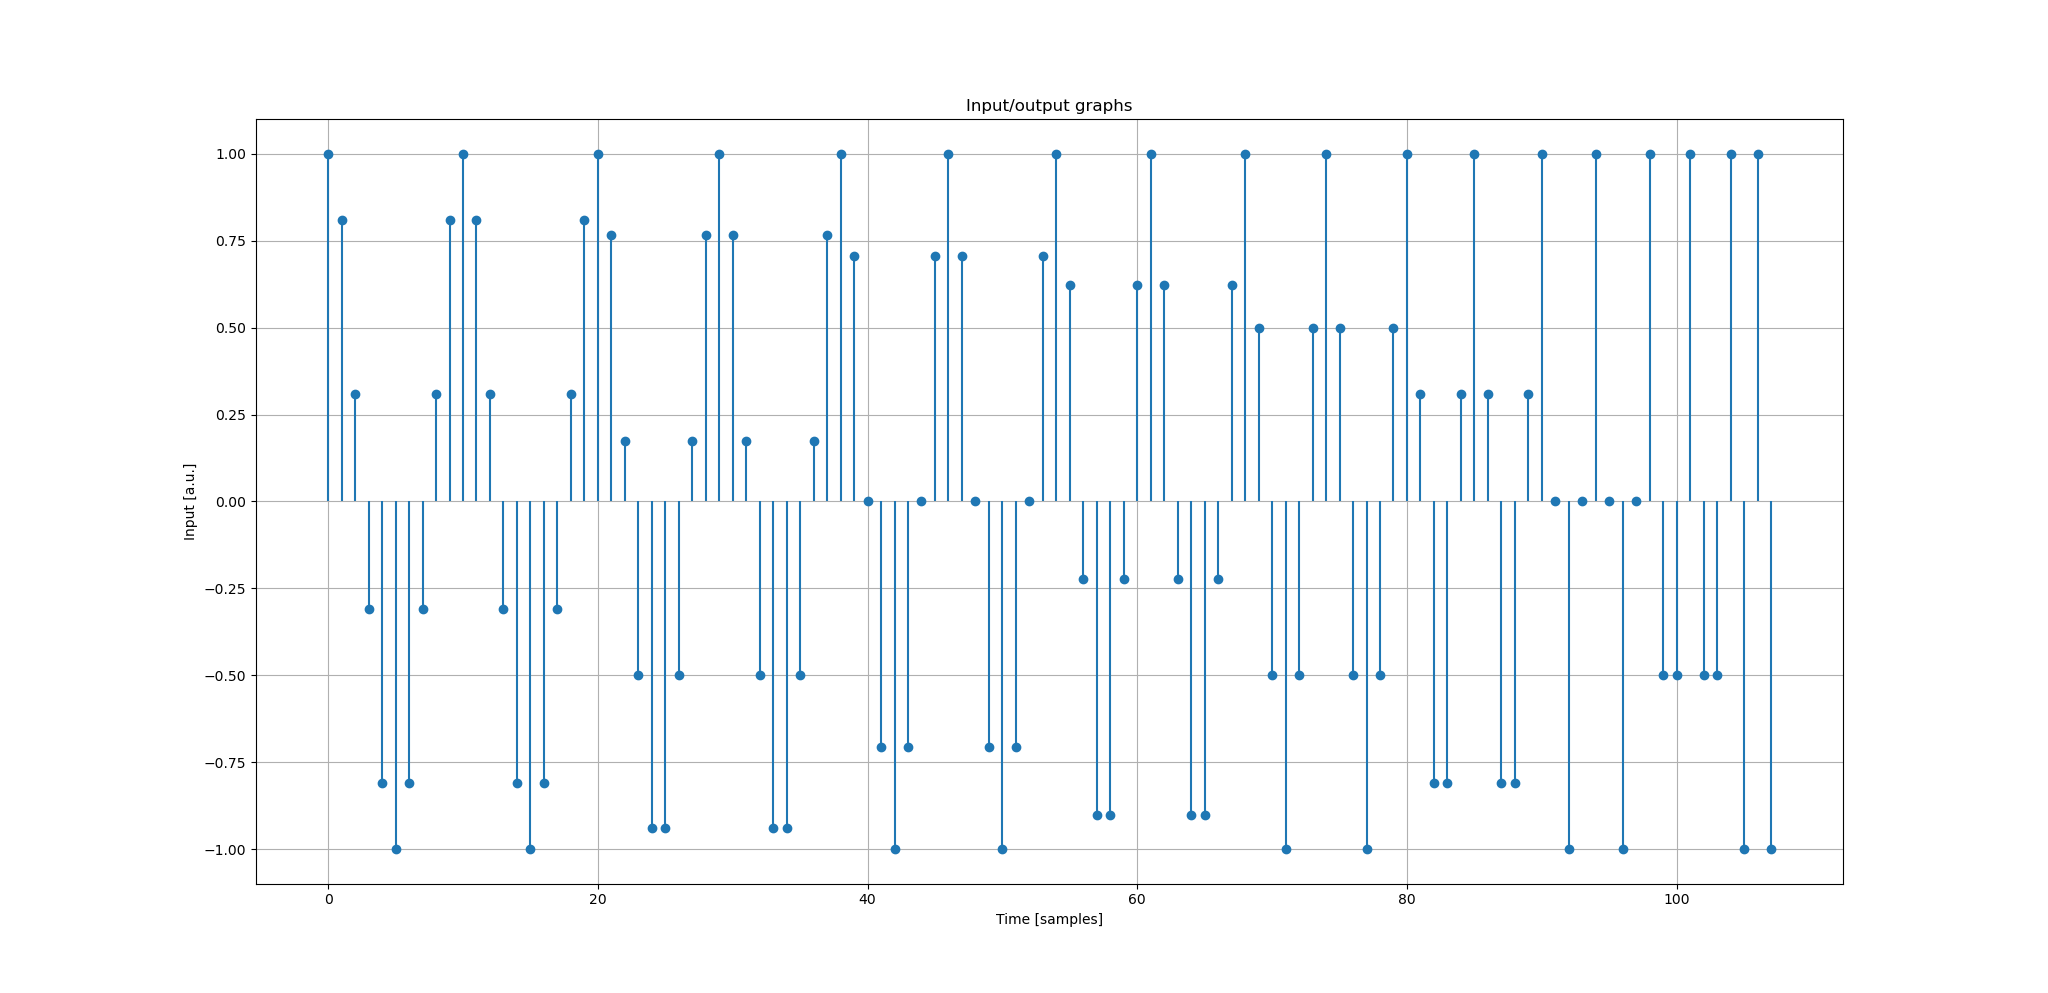
\includegraphics[scale=0.25]{figures/cos_sweep_N_10_to_N_2_P_2.PNG}
  \caption{Geração de um trem de cossenos, partindo do período $N=10$ até $N=2$, com 2 períodos por frequência.}\label{fig:cos_sweep_N_10_to_N_2_P_2}
\end{figure}

Decidiu-se utilizar o período em detrimento da frequência dada a grande dificuldade na manipulação de incrementos de frequência. Observamos problemas como os das figuras \ref{fig:bias_freq_next_to_pi_sweep} e \ref{fig:bias_freq_next_to_pi}

\begin{figure}[H]
  \centering
  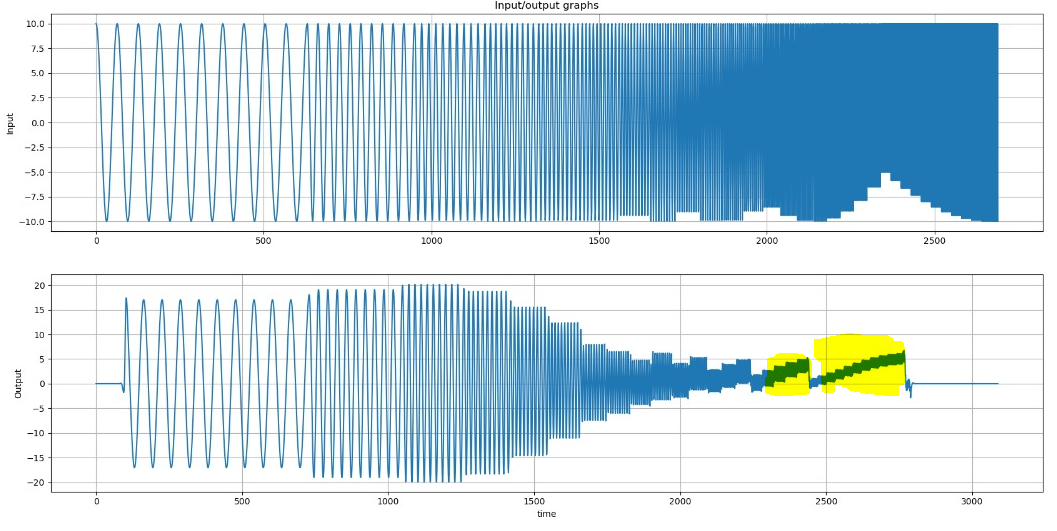
\includegraphics[scale=0.25]{figures/bias_freq_next_to_pi_sweep.PNG}
  \caption{Saída anômala durante a identificação por suposta falta de periodicidade do sinal.}\label{fig:bias_freq_next_to_pi_sweep}
\end{figure}

\begin{figure}[H]
  \centering
  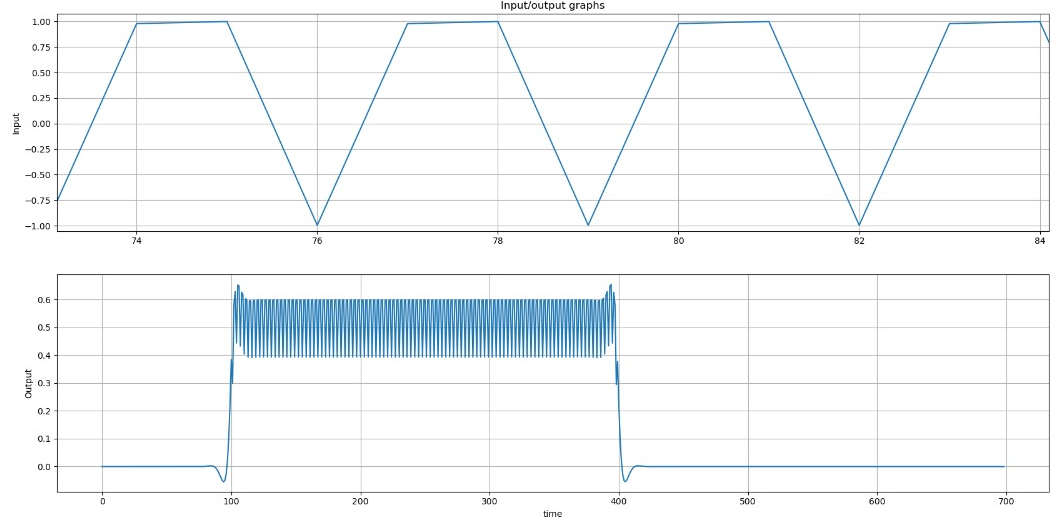
\includegraphics[scale=0.25]{figures/bias_freq_next_to_pi.PNG}
  \caption{Testes para análise em detalhes, deslocamento da saída por suposta falta de periodicidade do sinal. Observe que os platôs nos picos superiores do sinal estão apenas conectando um período ao próximo, mas essa conexão é inválida, uma vez que o período para essa frequência não é um inteiro.}\label{fig:bias_freq_next_to_pi}
\end{figure}

Chegamos a conclusão que o método de incremento de frequências estava se tornando complicado ao tentar encontrar frequências para as quais o sinal era periódico. Quando temos períodos não inteiros, aparentemente a média do sinal não é nula, injetando um nível contínuo (CC) no sistema. A definição da frequência se deu então pelo período, fazendo $k=1$ na equação de garantia do sinal periódico

\begin{equation}
  \omega=\frac{2\pi k}{N}=\frac{2\pi}{N}
\end{equation}

e assim conseguimos garantir que o sinal de saída, como o apresentado na figura \ref{fig:cos_sweep_N_10_to_N_2_P_2}, não possua a deriva observada em amarelo na \ref{fig:bias_freq_next_to_pi_sweep}. A confecção do vetor de frequências de excitação a partir dos períodos é dada na última linha do construtor da classe da biblioteca

\begin{minted}{python}
  def __init__(self, max_period, min_period, generate_periods):
      self.max_period = max_period
      self.min_period = min_period
      self.generate_periods = generate_periods
      self.periods = np.arange(self.max_period, self.min_period-1, -1)
      self.frequencies = 2*np.pi/self.periods
\end{minted}

Os parâmetros do usuário são passados para a instância da classe no código de execução

\begin{minted}{python}
  ## Instantiate system identification class
  #   Maximum period = 100
  #   Minimum period = 2
  #   Periods in each frequency = 100
  sys_idn = system_identification(100, 2, 100)
\end{minted}

e a construção do sinal se dá pela seguinte função

\begin{minted}{python}
  # Generate cosine "sweep" system input
  x = sys_idn.input_generator()
\end{minted}

O fato de possuirmos um computador digital impede que criemos um sinal de cosseno infinito, como idealizado pela teoria. Com isso, ocorre um transiente, na aplicação abrupta do sinal, visto que o sinal a esquerda do zero é zero desde $-\infty$. Para contornar esse problema, eliminamos as amostras iniciais da saída a fim de janelar um trecho em que o regime permanente já foi atingido. Isso foi discutido nas seções mencionadas (\ref{sssec:automated_procedure} e \ref{sssec:manual_procedure}) e, no código final, eliminamos um número de períodos definidos pelo usuário, o qual deverá analisar as saídas e verificar se aquele número foi suficientemente grande para a eliminação do transiente. A geração de diversos períodos no sinal de entrada também faz parte dessa eliminação do regime transitório, uma vez que o sistema permanece um tempo sendo excitado por uma única frequência.

A entrada passa pelo sistema e seu resultado é pós processado pelos seguintes trechos do código de execução

\begin{minted}{python}
  # Get the system output from our input
  y = sistema_desconhecido(x)

  ## Get the frequency respose
  #   Eliminate first 99 periods per frequency for each frequency to eliminate transitory response
  H = sys_idn.output_processor(y, 99)
\end{minted}

São eliminadas os 99 primeiros períodos de cada frequência dos 100 gerados. Isso foi suficiente para uma boa identificação e, aumentar esses números não trouxe melhoras significativas. Os trechos de código seguintes são referentes a plotagem dos gráficos e serão omitidos, no entanto, a figura \ref{fig:frequency_response} sintetiza e apresenta os resultados de todo o procetimento.

\begin{figure}[H]
  \centering
  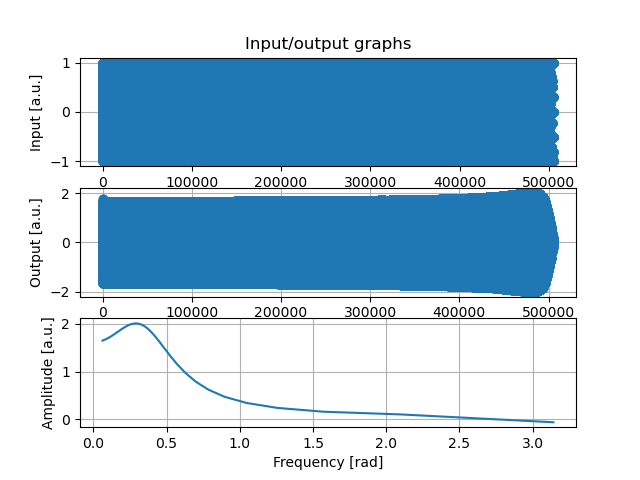
\includegraphics[scale=0.7]{figures/frequency_response.png}
  \caption{Gráficos da entrada, saída e resposta em frequência do sistema.}\label{fig:frequency_response}
\end{figure}

O intervalo requisitado pelo enunciado está compreendido,

Um ponto de grande discussão foi a medição da amplitude do sinal de saída. Extraímos o valor máximo do período seguinte do descarte e isso, por hipótese, pareceu suficiente dado que todo período contempla o valor máximo por cada trecho ser um sinal periódico, garantido por sua geração.



\end{document}
